\chapter[Multiscale Analysis of the Ictal Transition]{Multiscale Analysis of the\\Ictal Transition}
\label{chap:results}

Having established the theoretical observables in Chapter~\ref{chap:introduction} and the data-driven preprocessing pipeline in Chapter~\ref{chap:methods}, we now present the empirical investigation of the pre-ictal to ictal transition. We structure this chapter as a progressive multiscale zoom—moving from the macroscopic global graph, through mesoscopic community organization, down to microscopic node trajectories and functional role mapping. At each scale, we pair the core numerical implementation with the resulting dynamical profiles, concluding with a critical assessment of the methodological limitations that motivate the transition to the next scale of resolution.

Before decomposing the transition into specific topological metrics, it is instructive to inspect the raw structure of the signed dynamic functional connectivity tensor $\mathbf{W}(\tau) \in [-1, 1]^{N \times N}$ directly. Figure~\ref{fig:signed_overview} provides a panoramic overview of the connectivity matrices at three milestone time instants—Pre-Ictal ($t = -60.0\text{ s}$), Seizure Onset ($t = 0.0\text{ s}$), and Established Ictal ($t = +20.0\text{ s}$)—alongside the continuous temporal evolution of active cooperative links ($W_{ij} \geq 0.55$) and competitive anticorrelated links ($W_{ij} \leq -0.35$).

The three matrix snapshots in the top row of Figure~\ref{fig:signed_overview} visually justify the core methodological premises of this work:
\begin{itemize}
    \item \textbf{Pre-Ictal Baseline ($t = -60.0\text{ s}$):} The correlation matrix is dominated by pale, near-zero background values ($W_{ij} \approx 0$), with strong positive correlations restricted to small, block-diagonal squares along the main diagonal. These local blocks correspond to contacts situated along the same stereotactic depth electrode shaft, reflecting physiological local segregation and spatial volume conduction.
    \item \textbf{Seizure Onset Bifurcation ($t = 0.0\text{ s}$):} Exactly at the aligned transition point, off-diagonal structure erupts across the matrix. Crucially, the matrix does not turn uniformly red: instead, a striking checkerboard pattern of intense red blocks ($W_{ij} > +0.75$) and deep blue stripes ($W_{ij} < -0.60$) emerges. This confirms that as the ictal core locks into in-phase synchronization, specific subsets of channels simultaneously enter strong counter-phase opposition against the rest of the cortex. Had we applied the conventional absolute value rectification $\vert{}W_{ij}\vert{}$, these blue counter-phase stripes would have been folded into positive weights, completely obscuring the competitive geometry of the transition.
    \item \textbf{Established Ictal State ($t = +20.0\text{ s}$) and Global Density Evolution:} By $t = +20.0\text{ s}$, massive red off-diagonal blocks span almost the entire matrix, interrupted only by a few persistent blue counter-phase bands (around channel indices $35\text{--}45$). Consistently, the bottom panel shows that both cooperative links (blue curve) and anticorrelated links (red curve) remain low and stable ($\sim 3\text{--}10\%$) throughout the entire pre-ictal period, before jumping sharply at $t = 0\text{ s}$ into a sustained, high-density regime ($20\text{--}42\%$) that persists throughout the seizure.
\end{itemize}

\begin{figure}[htbp]
    \centering
    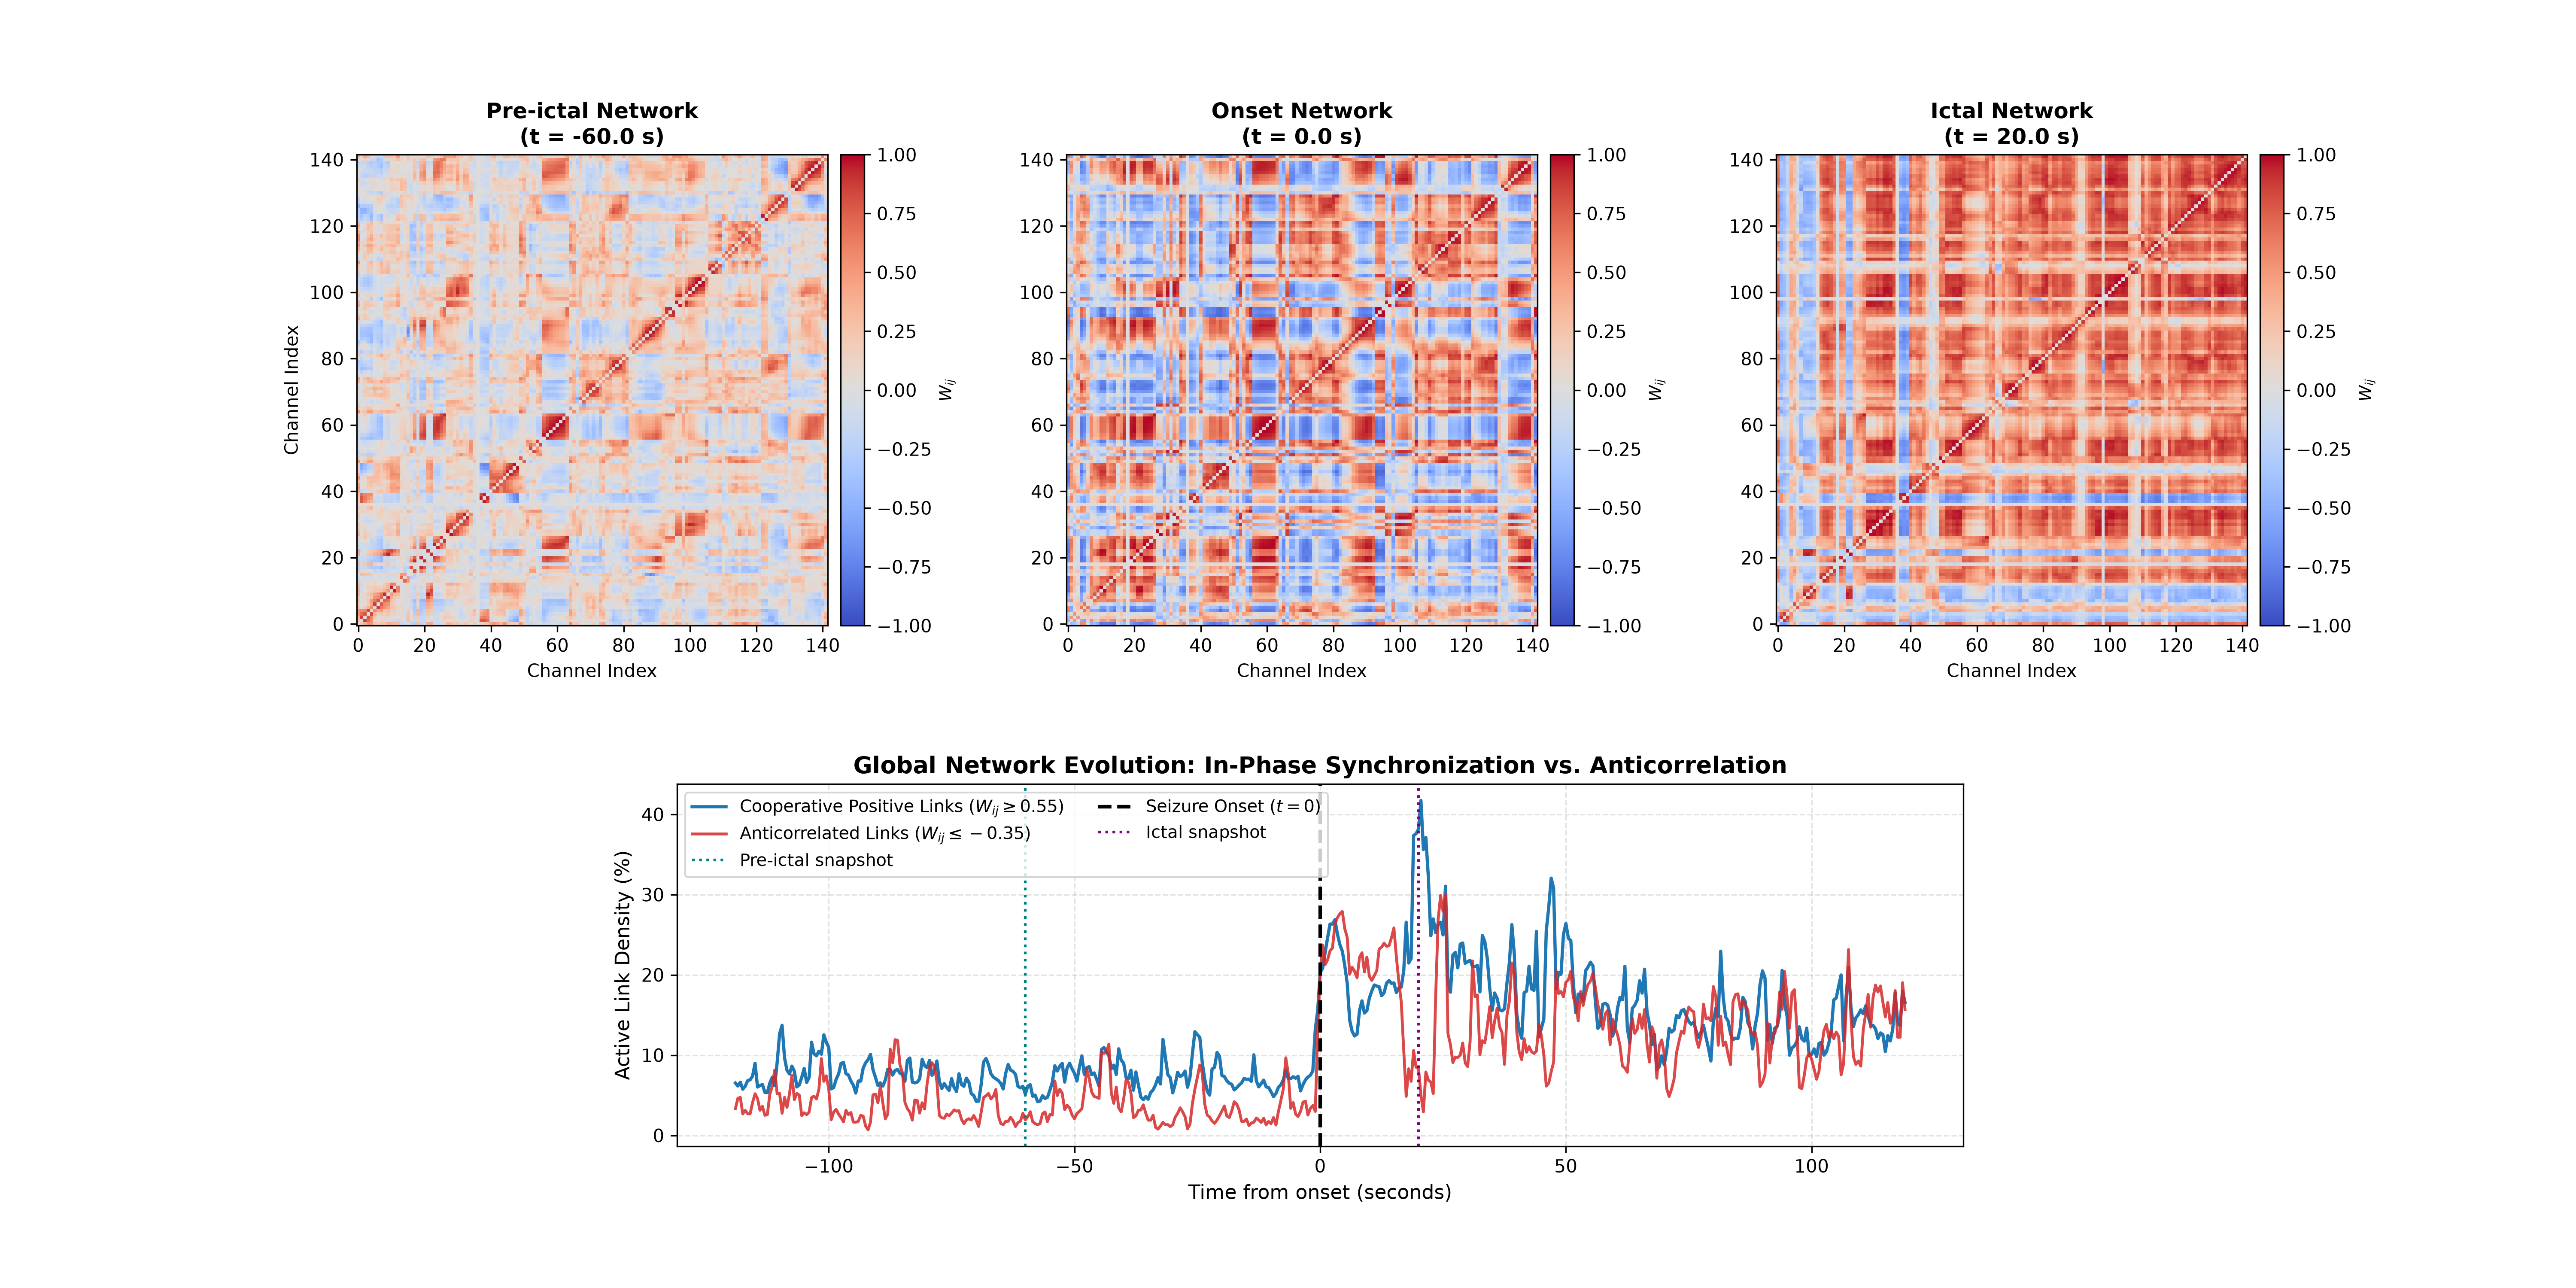
\includegraphics[width=0.9\textwidth]{img/DB470450/signed_connectivity_overview.png}
    \caption{Panoramic overview of the signed dynamic functional connectivity tensor $\mathbf{W}(\tau)$. Top row: Full $N \times N$ correlation matrices ($N \approx 140$ intracranial channels) sampled during the pre-ictal baseline ($t = -60.0\text{ s}$), seizure onset ($t = 0.0\text{ s}$), and established ictal propagation ($t = +20.0\text{ s}$). Warm colors ($W_{ij} > 0$, red) denote in-phase cooperative synchronization; cool colors ($W_{ij} < 0$, blue) denote counter-phase anticorrelation. Bottom panel: Global temporal evolution of the active cooperative link density ($W_{ij} \geq 0.55$, blue trace) versus competitive anticorrelated link density ($W_{ij} \leq -0.35$, red trace) across the $240\text{ s}$ window.}
    \label{fig:signed_overview}
\end{figure}
With this global intuition established, we now proceed to quantify the transition systematically across the three topological scales on our reference recording (\texttt{DB470450}), followed by a cross-patient robustness analysis in Section~\ref{sec:cohort_robustness}.

\section{Macroscopic Scale: Percolation Phase Transition and Critical Susceptibility}
\label{sec:act1_macro}

\subsection{Physical Motivation}
At the coarsest level of resolution, our primary question is whether the onset of a focal seizure manifests macroscopically as a collective phase transition. During the physiological inter-ictal baseline, functional coupling between distinct sEEG contacts is expected to remain weak, transient, and spatially localized, keeping the global graph in a fragmented, subcritical regime. As the epileptogenic zone overcomes local inhibitory restraint at $t = 0\text{ s}$, we test whether the cortical network undergoes a percolation transition characterized by: (i) the sudden macroscopic emergence of a Giant Connected Component $S(\tau)$, (ii) a sharp divergence in topological susceptibility $\chi(\tau) = \text{Var}(k(\tau))$ marking critical degree heterogeneity, and (iii) a global divergence between cooperative in-phase synchronization and competitive counter-phase decoupling.

\subsection{Numerical Implementation}
To evaluate percolation metrics across the $T_{\text{wins}} = 477$ sliding windows without introducing spatial priors, each frame $\mathbf{W}(\tau)$ of the signed connectivity tensor is thresholded at the calibrated critical value $\theta$ ($\theta = 0.50$ for \texttt{DB470450}). The size of the Giant Connected Component $N_{\text{GCC}}(\tau)$ is extracted via breadth-first graph traversal on the sparse binary adjacency matrix $\mathbf{A}(\tau)$, while the susceptibility $\chi(\tau)$ and the positive/negative edge densities ($D^{+}(\tau)$ for $W_{ij} \geq \theta$ and $D^{-}(\tau)$ for $W_{ij} \leq \theta_{\text{neg}} = -0.35$) are computed directly from the upper triangular entries of $\mathbf{W}(\tau)$:

\begin{lstlisting}[language=Python, caption={Macroscopic percolation metrics: Giant Connected Component $S(\tau)$, topological susceptibility $\chi(\tau)$, and signed edge densities.}]
from scipy.sparse import csr_matrix
from scipy.sparse.csgraph import connected_components

def compute_macroscopic_percolation(W, pos_thresh=0.50, neg_thresh=-0.35):
    n_wins, n_nodes, _ = W.shape
    triu_idx = np.triu_indices(n_nodes, k=1)
    n_pairs = len(triu_idx[0])

    gcc_fraction = np.zeros(n_wins, dtype=np.float64)
    susceptibility = np.zeros(n_wins, dtype=np.float64)
    pos_density = np.zeros(n_wins, dtype=np.float64)
    neg_density = np.zeros(n_wins, dtype=np.float64)

    for t in range(n_wins):
        W_t = W[t]
        upper_vals = W_t[triu_idx]

        # Global cooperative vs. competitive edge densities
        pos_density[t] = np.sum(upper_vals >= pos_thresh) / n_pairs
        neg_density[t] = np.sum(upper_vals <= neg_thresh) / n_pairs

        # Binary cooperative adjacency matrix A(t)
        adj = (W_t >= pos_thresh).astype(np.int8)
        np.fill_diagonal(adj, 0)

        # Connected components via sparse breadth-first search
        n_comp, labels = connected_components(csr_matrix(adj), directed=False)
        _, counts = np.unique(labels, return_counts=True)
        gcc_fraction[t] = np.max(counts) / float(n_nodes)

        # Topological susceptibility as spatial degree variance Var(k)
        degrees = np.sum(adj, axis=1)
        susceptibility[t] = np.var(degrees)

    return gcc_fraction, susceptibility, pos_density, neg_density
\end{lstlisting}

\subsection{Empirical Results: Multi-Threshold Percolation and Susceptibility}
Figure~\ref{fig:act1_percolation} illustrates the macroscopic percolation transition across the $[-120\text{ s}, +120\text{ s}]$ window by comparing the evolution of the Giant Connected Component $S(\tau)$ (top panel) and the topological susceptibility $\chi(\tau) = \text{Var}(k(\tau))$ (bottom panel) across three distinct binarization thresholds: $\theta \in \{0.40, 0.50, 0.65\}$.

\begin{figure}[htbp]
    \centering
    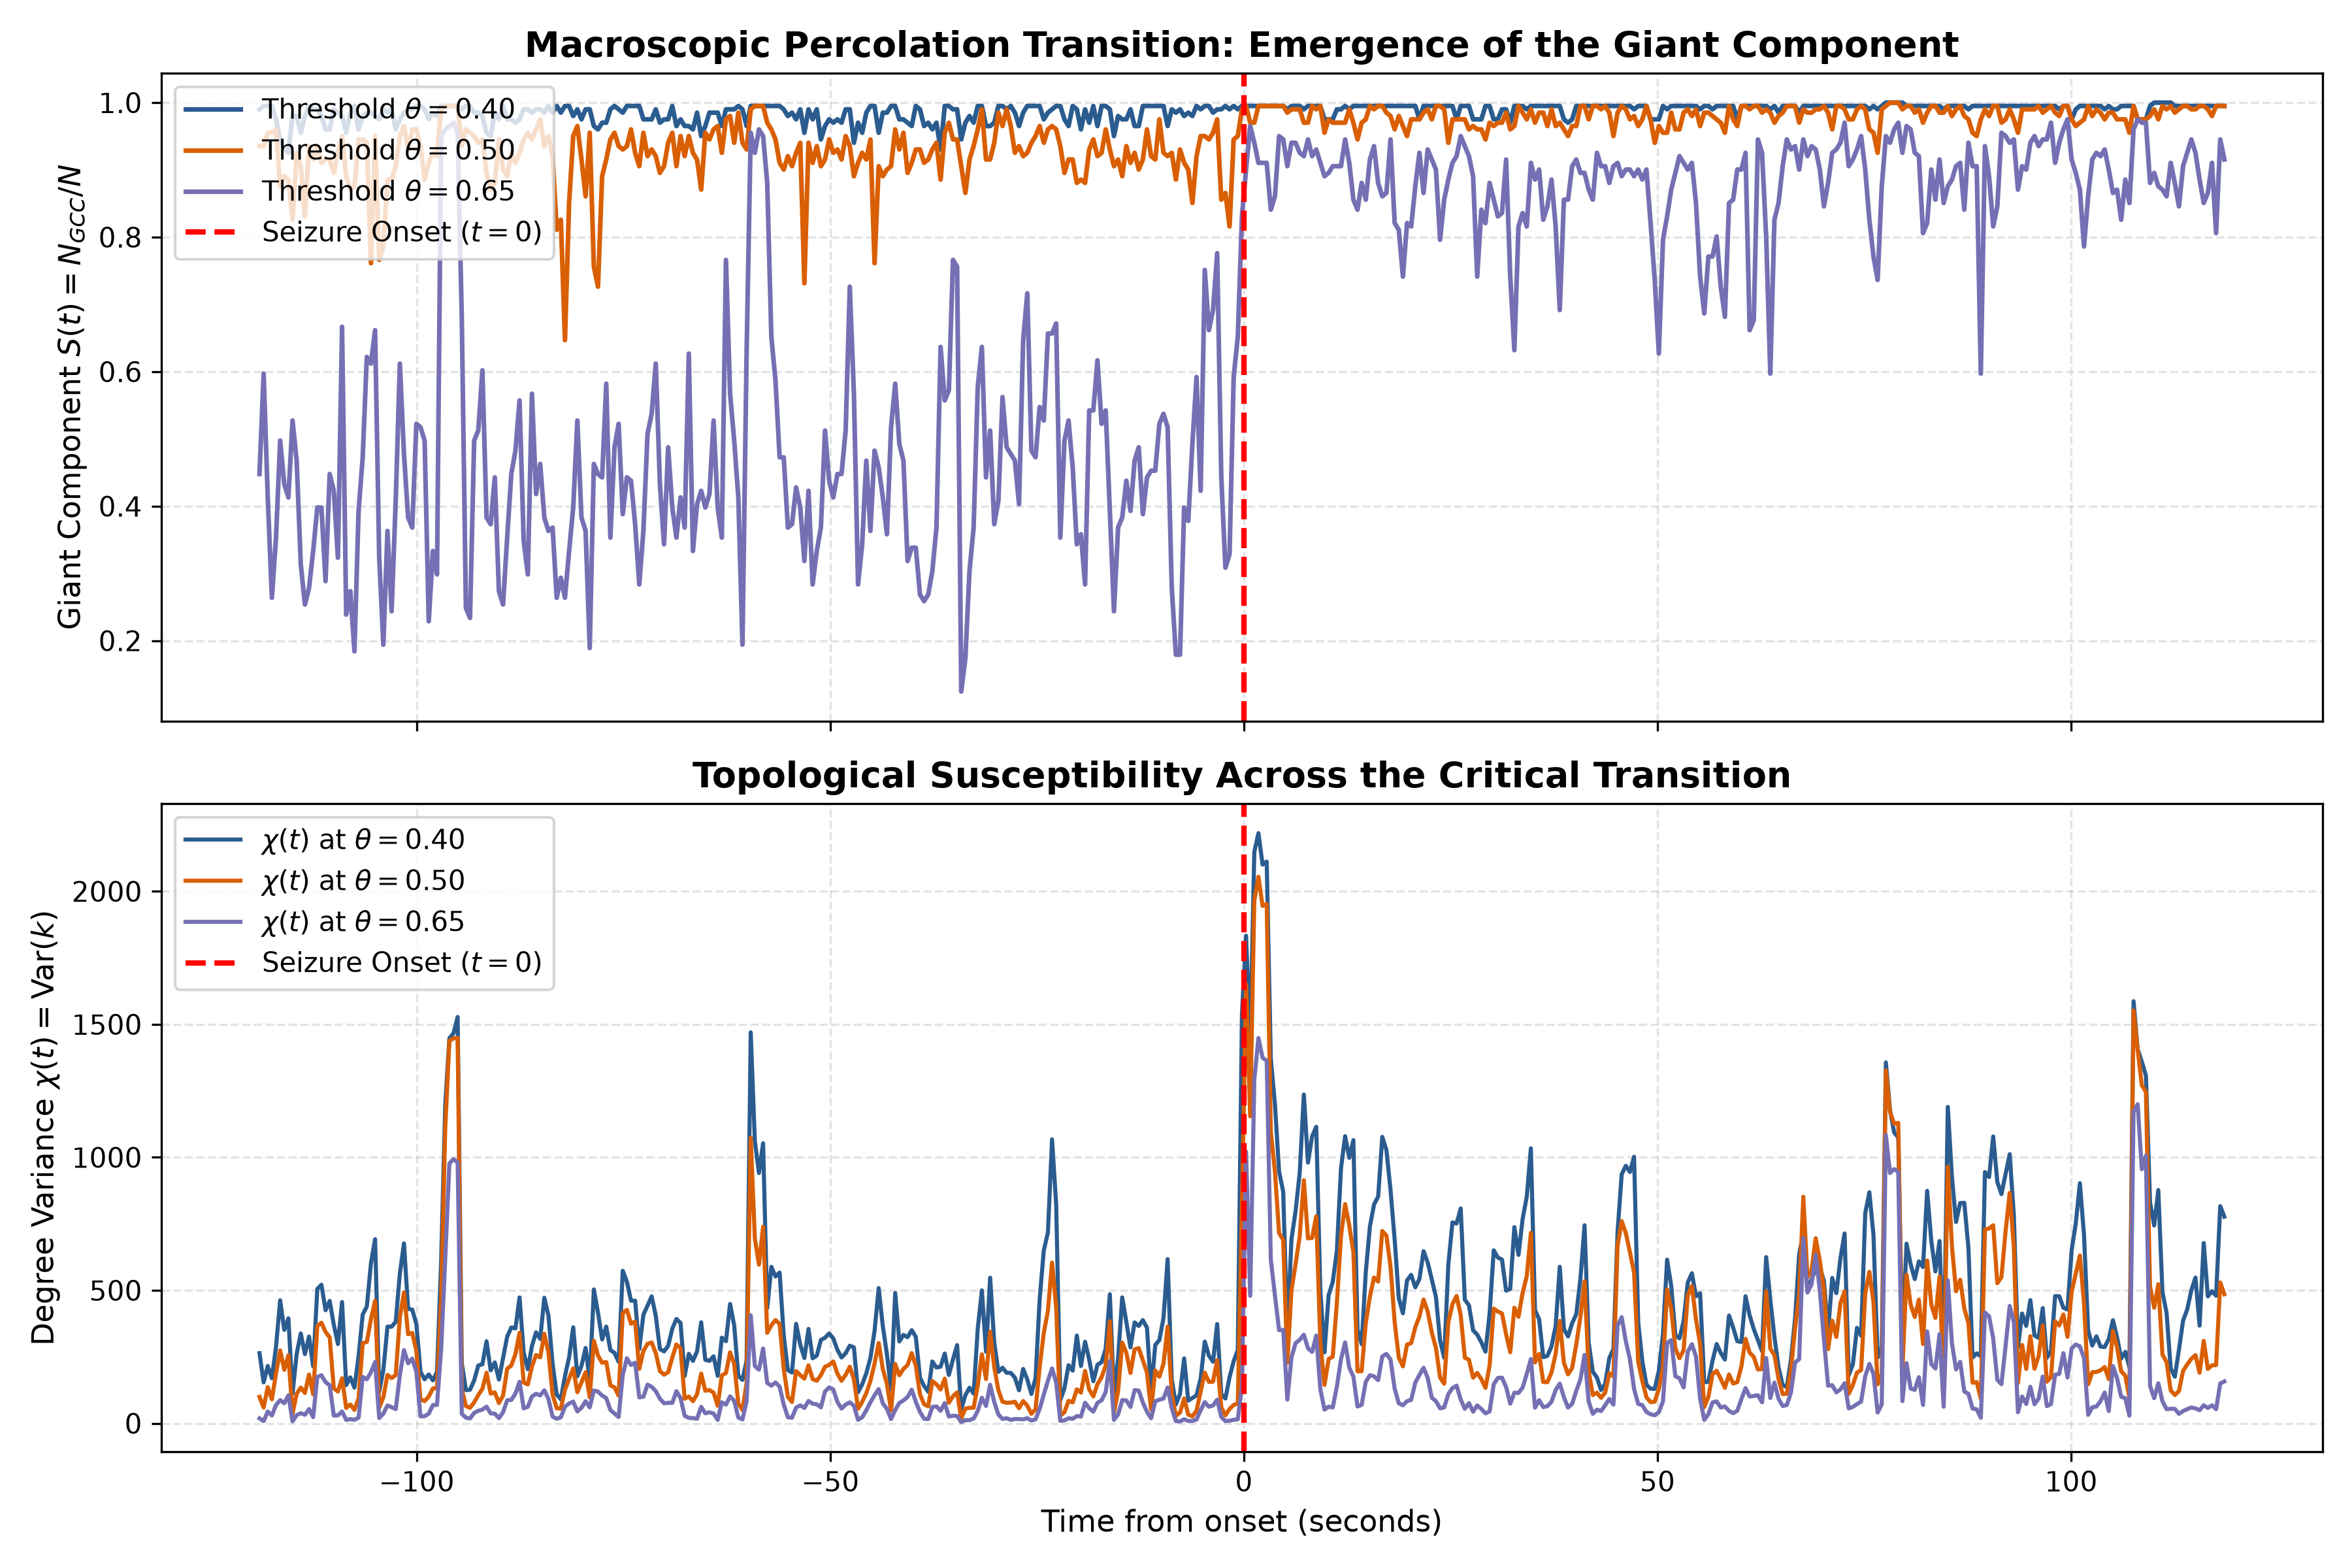
\includegraphics[width=0.9\textwidth]{img/DB470450/macro_percolation_transition.png}
    \caption{Macroscopic percolation transition across correlation thresholds $\theta \in \{0.40, 0.50, 0.65\}$. Top: Normalized Giant Connected Component size $S(\tau) = N_{\text{GCC}}/N$. Bottom: Topological susceptibility $\chi(\tau) = \text{Var}(k(\tau))$ peaking sharply at the aligned seizure onset ($t = 0\text{ s}$, red dashed line).}
    \label{fig:act1_percolation}
\end{figure}

Comparing the three curves in the top panel of Figure~\ref{fig:act1_percolation} provides a textbook demonstration of how the choice of the control parameter $\theta$ determines the observability of the percolation phase transition:
\begin{itemize}
    \item \textbf{Supercritical Saturation at Low Thresholds ($\theta = 0.40$ and $\theta = 0.50$):} For permissive thresholds (blue and orange traces), background physiological correlations and volume conduction are sufficient to maintain a spanning tree across the electrode array even during the inter-ictal baseline. Consequently, $S(\tau)$ remains pinned near $0.95\text{--}1.0$ for $\theta = 0.40$ and fluctuates high between $0.80$ and $0.98$ for $\theta = 0.50$, largely masking the macroscopic jump at seizure onset.
    \item \textbf{Critical Percolation Regime ($\theta = 0.65$):} Raising the threshold to a stringent level ($\theta = 0.65$, purple trace) prunes weak background links and places the pre-ictal network genuinely within the \textit{subcritical fragmented phase}, where $S(\tau)$ fluctuates broadly between $0.20$ and $0.65$. Exactly at the aligned electrophysiological onset ($t = 0\text{ s}$), the network undergoes a sharp discontinuous transition: $S(\tau)$ jumps to $\sim 0.95\text{--}1.0$ and remains stably in the percolating regime ($S(\tau) \in [0.80, 0.98]$) throughout the subsequent ictal propagation.
\end{itemize}

Remarkably, the bottom panel of Figure~\ref{fig:act1_percolation} reveals that while $S(\tau)$ is prone to ceiling saturation at lower thresholds, the topological susceptibility $\chi(\tau) = \text{Var}(k(\tau))$ acts as a threshold-robust indicator of criticality. During the quiet baseline, $\chi(\tau)$ remains low ($\chi < 400$ across all thresholds), interrupted only by two brief, isolated inter-ictal bursts at $\tau \approx -95\text{ s}$ ($\chi \approx 1500$) and $\tau \approx -59\text{ s}$ ($\chi \approx 1450$), where transient synchronization spikes and rapidly relaxes due to intact cortical inhibition. Exactly at seizure onset ($t \in [0, +3]\text{ s}$), however, $\chi(\tau)$ exhibits its absolute global maximum across all thresholds simultaneously—surging to $\chi \approx 2250$ for $\theta = 0.40$, $\chi \approx 2050$ for $\theta = 0.50$, and $\chi \approx 1450$ for $\theta = 0.65$. Physically, this sharp divergence in degree variance captures the critical spatial heterogeneity at the bifurcation point, where a hyper-connected core of ictal hub channels coexists with still-unrecruited peripheral contacts before the seizure settles into a fluctuating ictal plateau.

\subsection{Critical Assessment and Limitations of the Macroscopic View}
While $S(\tau)$ and $\chi(\tau)$ confirm that seizure onset obeys the phenomenology of a critical percolation transition, relying exclusively on macroscopic binary descriptors presents two significant limitations:
\begin{enumerate}
    \item \textbf{Threshold Sensitivity:} Both $S(\tau)$ and $\chi(\tau)$ depend on the choice of the binarization threshold $\theta$. If $\theta$ is set too low (e.g., $\theta < 0.35$), weak background correlations already percolate into a giant component during the inter-ictal state ($S(\tau) \approx 1$ everywhere), masking the onset jump. Conversely, if $\theta$ is set too high ($\theta > 0.75$), the graph remains fragmented even during the seizure. Although our data-driven calibration (targeting a subcritical baseline density of $\sim 7\%$) mitigates this arbitrariness, a threshold-free validation of network coalescence is desirable.
    \item \textbf{Topological Blindness to Internal Structure:} Once $S(\tau)$ saturates near $1$, percolation theory only tells us that a path exists between almost all nodes. It cannot distinguish whether the graph consists of several loosely connected functional modules (connected by a few bridge edges) or a genuinely collapsed, homogeneous syncytium.
\end{enumerate}
To overcome threshold dependence and resolve the internal reorganization of functional subsystems, we must move to the mesoscopic scale.

\section{Mesoscopic Scale: Community Reorganization and Modularity Collapse}
\label{sec:act2_meso}

\subsection{Physical Motivation}
As demonstrated in the macroscopic analysis, observing $S(\tau) \to 1$ at lower thresholds ($\theta \leq 0.55$) indicates that a path connects almost all nodes in the graph, yet it leaves open a fundamental topological question: does the pre-ictal network consist of distinct, weakly coupled functional modules that only merge into a single dense syncytium at $t = 0\text{ s}$?

To resolve this internal architecture, we move to the mesoscopic scale. In a healthy physiological state, cortical computation relies on functional segregation, which manifests graph-theoretically as a high Newman Modularity $Q(\tau)$ and a large number of autonomous communities $N_c(\tau)$. We hypothesize that the onset of the epileptic seizure induces a mesoscopic collapse, i.e. a sudden drop in $Q(\tau)$ accompanied by the coalescence of multiple pre-ictal modules into a minimal number of macro-communities dominated by the pathological Giant Component.

\subsection{Numerical Implementation}
For each sliding window $\tau$, we construct the thresholded positive weighted graph $W_{ij}^{(\theta)}(\tau) = W_{ij}(\tau) \, \Theta(W_{ij}(\tau) - \theta)$ at the calibrated mesoscopic threshold $\theta = 0.55$. Retaining the continuous weights $W_{ij}(\tau) \geq \theta$ preserves the relative interaction strengths within the active backbone while suppressing background correlation noise. We then apply the Louvain heuristic algorithm to extract the optimal partition $\mathcal{C}(\tau)$, recording both the maximum modularity score $Q(\tau)$ according to Equation~(\ref{eq:modularity}) and the total number of detected communities $N_c(\tau) = |\mathcal{C}(\tau)|$:

\begin{lstlisting}[language=Python, caption={Mesoscopic community detection via the Louvain algorithm and Newman's weighted modularity $Q(\tau)$.}]
import networkx as nx
from networkx.algorithms.community import louvain_communities, modularity

def compute_mesoscopic_modularity(W, threshold=0.55, seed=42):
    n_wins, n_nodes, _ = W.shape
    modularity_q = np.zeros(n_wins, dtype=np.float64)
    n_communities = np.zeros(n_wins, dtype=np.int32)

    for t in range(n_wins):
        # Thresholded positive weighted adjacency matrix
        W_pos = np.where(W[t] >= threshold, W[t], 0.0)
        np.fill_diagonal(W_pos, 0.0)

        G = nx.from_numpy_array(W_pos)
        if G.size(weight="weight") == 0:
            n_communities[t] = n_nodes
            modularity_q[t] = 0.0
            continue

        # Louvain community partitioning and Newman's Q evaluation
        communities = louvain_communities(G, weight="weight", seed=seed)
        modularity_q[t] = modularity(G, communities, weight="weight")
        n_communities[t] = len(communities)

    return modularity_q, n_communities
\end{lstlisting}

\subsection{Empirical Results: Breakdown of Functional Segregation}
Figure~\ref{fig:act2_modularity} displays the temporal evolution of Newman's Modularity $Q(\tau)$ (top panel) and the total number of detected communities $N_c(\tau)$ (bottom panel) at $\theta = 0.55$.

\begin{figure}[htbp]
    \centering
    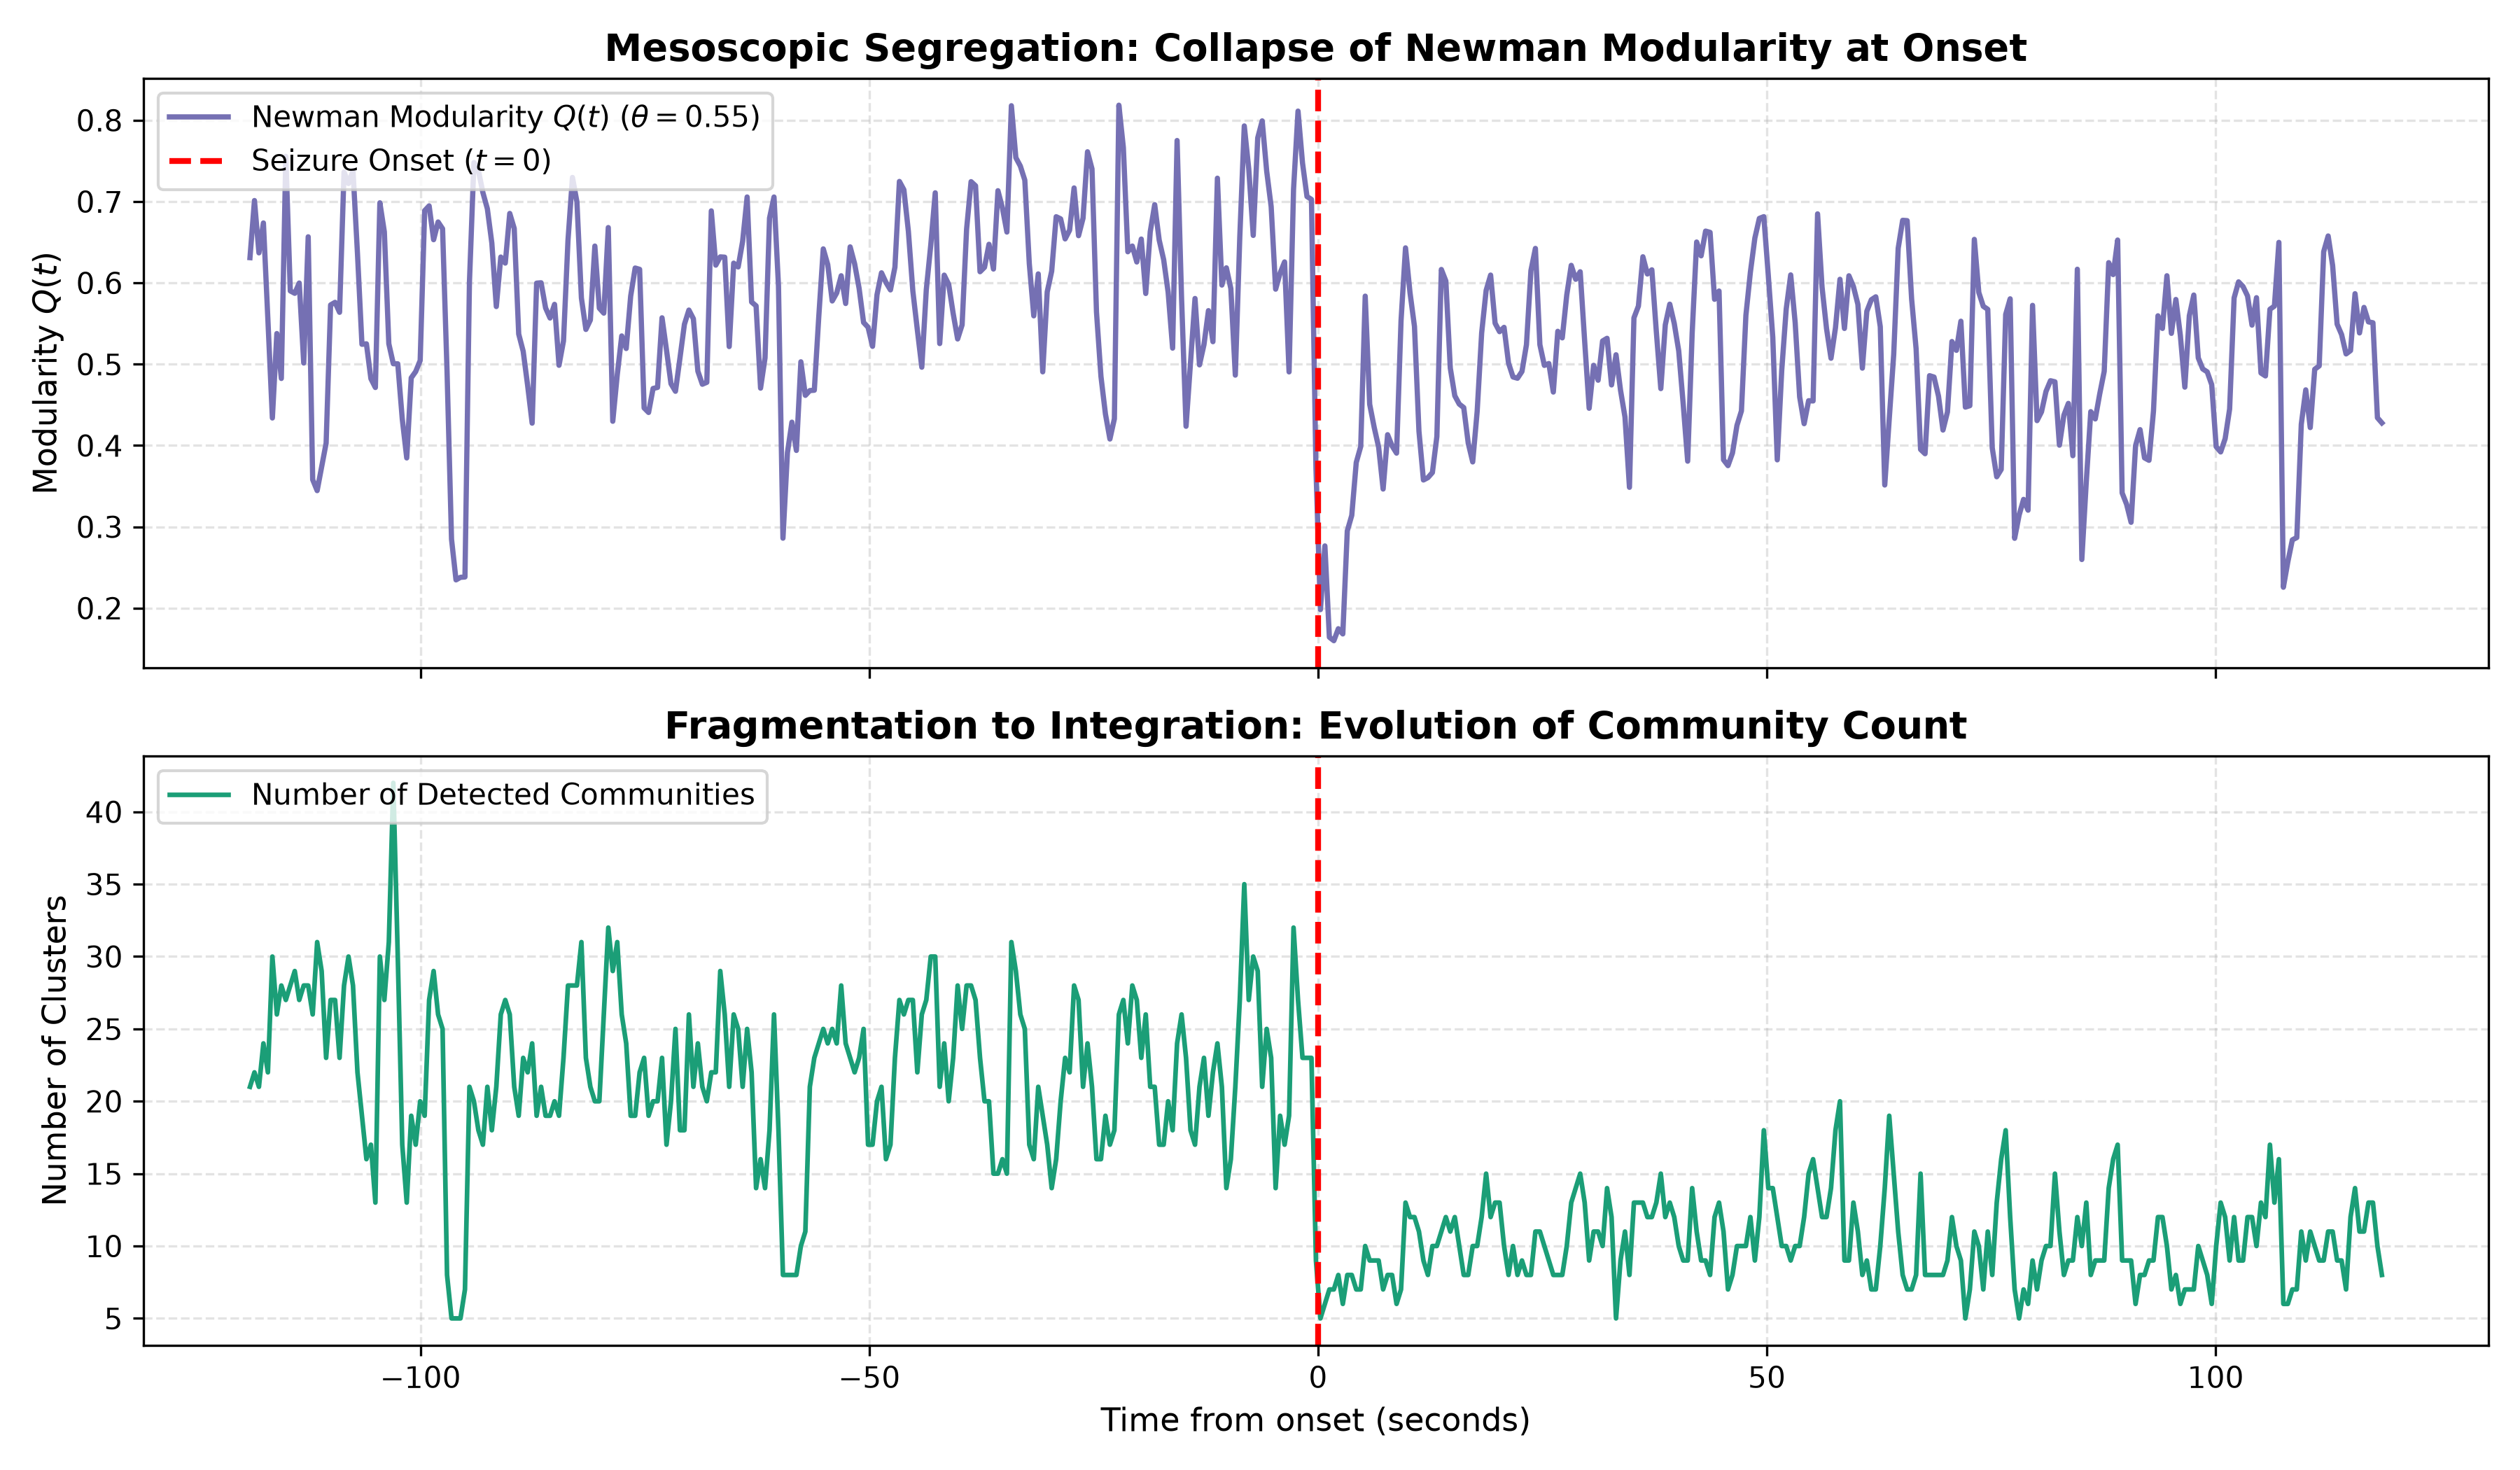
\includegraphics[width=0.9\textwidth]{img/DB470450/meso_modularity_collapse.png}
    \caption{Mesoscopic segregation dynamics across seizure onset ($\theta = 0.55$). Top: Evolution of Newman's weighted Modularity $Q(\tau)$, exhibiting a sharp collapse at $t = 0\text{ s}$. Bottom: Total number of detected Louvain communities $N_c(\tau)$, illustrating the abrupt transition from pre-ictal fragmentation to ictal integration.}
    \label{fig:act2_modularity}
\end{figure}

The mesoscopic time series in Figure~\ref{fig:act2_modularity} uncover a striking dynamical symmetry breaking that was partially hidden by ceiling effects in the macroscopic order parameter $S(\tau)$:
\begin{itemize}
    \item \textbf{Pre-Ictal Functional Segregation ($t < 0\text{ s}$):} Throughout the inter-ictal baseline, the cortical network maintains a highly segregated modular organization, with $Q(\tau)$ fluctuating around a high mean value of $Q \approx 0.60\text{--}0.75$ and the graph partitioned into $N_c(\tau) \approx 20\text{--}32$ distinct functional clusters. Notably, the two transient inter-ictal bursts previously observed in $\chi(\tau)$ at $\tau \approx -95\text{ s}$ and $\tau \approx -59\text{ s}$ appear here as brief, reversible dips where modularity drops ($Q \to 0.24$ and $0.29$) and communities momentarily coalesce ($N_c \to 5$ and $8$) before immediately rebounding to the segregated baseline.
    \item \textbf{Critical Modularity Collapse at Onset ($t = 0\text{ s}$):} Right across the premonitory window ($\tau \in [-15, 0]\text{ s}$), modularity reaches elevated values ($Q \approx 0.75\text{--}0.82$), reflecting strong local isolation prior to the transition. Exactly at $t = 0\text{ s}$, functional segregation collapses catastrophically: $Q(\tau)$ plummets within $2\text{ seconds}$ from $\sim 0.80$ down to its global minimum of $Q \approx 0.16$, while the number of communities drops precipitously from $N_c \approx 25\text{--}35$ down to just $N_c \approx 4\text{--}5$ clusters.
    \item \textbf{Post-Onset Ictal Reorganization ($t > +10\text{ s}$):} Following the acute onset collapse, the network does not return to its pre-ictal state. Instead, it settles into a new, persistently integrated ictal regime characterized by a permanently reduced community count ($N_c(\tau) \approx 8\text{--}15$, roughly half the pre-ictal baseline) and lower average modularity ($Q(\tau) \approx 0.45\text{--}0.55$).
\end{itemize}

To visualize this topological reorganization directly in graph space without relying on anatomical coordinates, Figure~\ref{fig:act2_snapshots} renders the network at three representative time snapshots using a force-directed Kamada-Kawai spring layout ($\theta = 0.55$), where nodes are colored by their Louvain community assignment.

\begin{figure}[htbp]
    \centering
    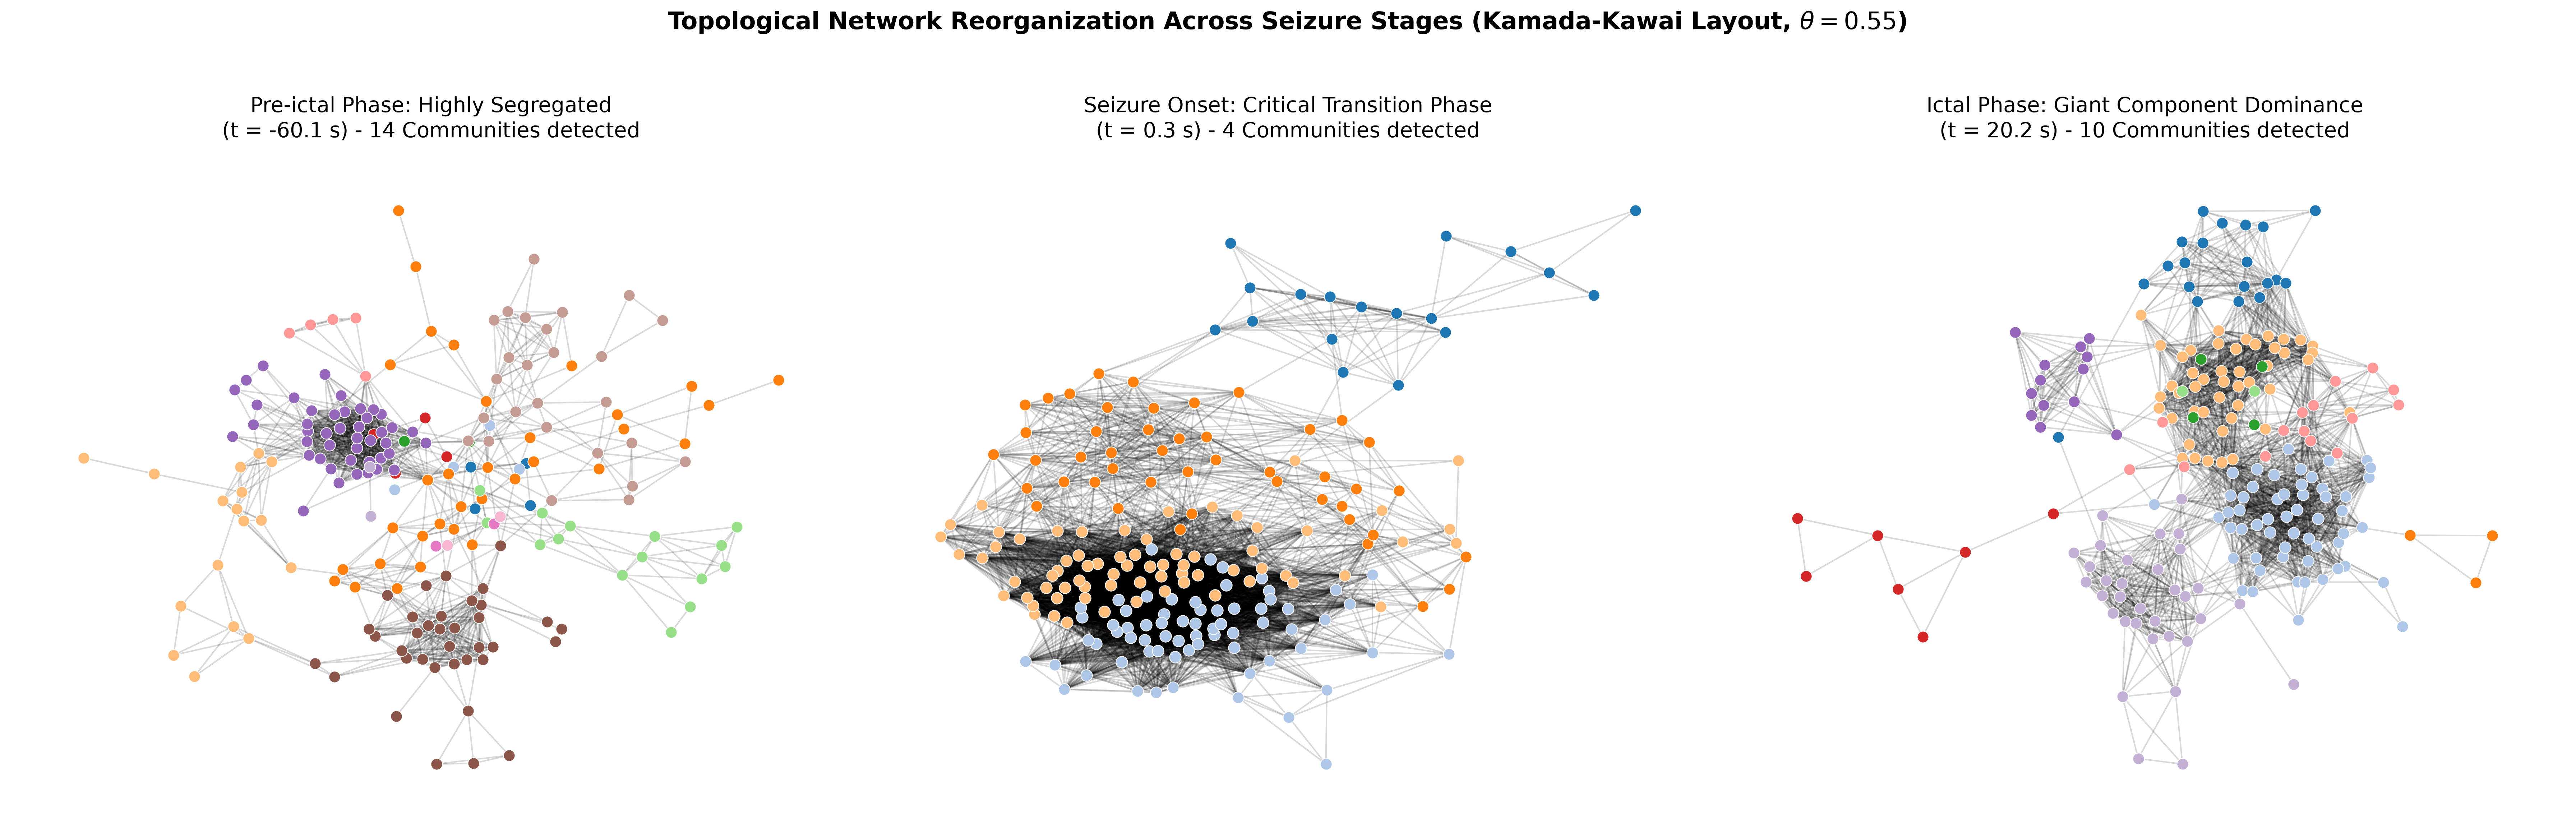
\includegraphics[width=0.9\textwidth]{img/DB470450/meso_community_topology_snapshots.png}
    \caption{Topological network reorganization across seizure stages rendered via force-directed Kamada-Kawai layout ($\theta = 0.55$, isolated singletons omitted for visual clarity). Left: Pre-ictal segregated state ($t = -60.1\text{ s}$, $14$ active multi-node communities). Center: Seizure onset critical transition ($t = +0.3\text{ s}$), where modules collapse into $4$ communities dominated by a dense hyper-synchronized core. Right: Established ictal phase ($t = +20.2\text{ s}$, $10$ communities) showing core-periphery reorganization.}
    \label{fig:act2_snapshots}
\end{figure}

In the pre-ictal snapshot ($t = -60.1\text{ s}$, left panel), the network exhibits a distributed web of $14$ loosely coupled communities (purple, brown, orange, and green clusters) with sparse inter-modular bridges. At seizure onset ($t = +0.3\text{ s}$, center panel), this modular hierarchy implodes: virtually all nodes are pulled into a massive, tightly bound central syncytium (light-blue and orange nodes) with only $4$ communities remaining. By the established ictal phase ($t = +20.2\text{ s}$, right panel), the giant component partially differentiates into two main coupled macro-lobes ($10$ communities total), matching the secondary rebound in $Q(\tau)$ observed in Figure~\ref{fig:act2_modularity}.

\subsection{Critical Assessment and Limitations of the Mesoscopic View}
While Newman's Modularity $Q(\tau)$ successfully resolves the internal breakdown of functional segregation at $t = 0\text{ s}$, mesoscopic community detection exhibits three methodological limitations that prevent it from answering our clinical question on its own:
\begin{enumerate}
    \item \textbf{Resolution Limit and Degeneracy of Louvain:} Modularity optimization suffers from a well-known resolution limit \cite{newman2018networks}: when total edge weight $2m(\tau)$ changes drastically across the transition, Louvain may merge small physiological modules or split large ictal clusters unpredictably, and its stochastic node-sweeping order produces slight frame-to-frame jitter in $Q(\tau)$.
    \item \textbf{Exclusion of Negative Anticorrelations:} Standard Newman modularity (Equation~\ref{eq:modularity}) is formulated strictly for non-negative edge weights $W_{ij}^{+} \geq 0$. Consequently, the mesoscopic view is completely blind to the competitive counter-phase decoupling ($W_{ij} < 0$) that precedes seizure onset.
    \item \textbf{Nodal Anonymity:} Knowing that $Q(\tau)$ collapses from $0.80$ to $0.16$ tells us \textit{that} the brain's modular barriers have broken down, but it does not identify \textit{which specific electrode contacts} initiated the decoupling prior to $t = 0\text{ s}$ or which contacts act as the primary hub drivers of the onset syncytium.
\end{enumerate}
To break nodal anonymity and incorporate the negative correlation spectrum, we must descend to the microscopic scale of individual channels.

\section{Microscopic Scale: Premonitory Decoupling and the 2D Functional Role Map}
\label{sec:act3_micro}

\subsection{Physical and Clinical Motivation}
Acts~I and~II demonstrated that seizure onset manifests globally as a critical percolation transition ($S(\tau) \to 1$, $\chi(\tau)$ peak) and mesoscopically as a sudden collapse of modular segregation ($Q(\tau) \to 0.16$). However, from both a dynamical systems and an epileptological perspective, the decisive question lies at the microscopic scale of individual nodes: \textit{which specific sEEG contacts drive this phase transition?}

In particular, guided by the clinical hypothesis of pre-ictal functional detachment \cite{jiruska2013synchronization, mormann2003epileptic}, we seek to verify whether contacts belonging to the putative epileptogenic network exhibit a premonitory decoupling phase—isolating themselves via negative anticorrelations ($W_{ij} < 0$) in the seconds immediately preceding $t = 0\text{ s}$, before recruiting the cortical network into the Giant Connected Component. Furthermore, by pairing pre-ictal decoupling with onset eigenvector centrality across calibrated statistical epochs, we aim to construct an objective two-dimensional classification of nodal roles.

\subsection{Numerical Implementation}
For each time window $\tau$, we characterize every node $i \in \{1, \dots, N\}$ along two complementary dimensions:
\begin{enumerate}
    \item \textbf{Signed Neighbourhood Correlation and Negative Decoupling:} From the unthresholded signed matrix $\mathbf{W}(\tau)$, we compute each node's mean signed correlation $\bar{W}_i(\tau) = \frac{1}{N-1}\sum_{j \neq i} W_{ij}(\tau)$ to track its net phase alignment, alongside its strictly negative decoupling score $d_i^{(-)}(\tau) = \frac{1}{N-1}\sum_{j \neq i} |\min(0, W_{ij}(\tau))|$ (Equation~\ref{eq:decoupling_score}).
    \item \textbf{Leading Eigenvector Centrality:} From the cooperative binary adjacency matrix $\mathbf{A}(\tau)$ (thresholded at the calibrated critical value $\theta = 0.55$), we extract the principal eigenvector $\mathbf{v}_1(\tau)$ associated with the largest eigenvalue $\lambda_1(\tau)$ via power iteration, normalized in the $L_1$-norm ($\sum_i v_{1,i}(\tau) = 1$) so that $v_{1,i}(\tau)$ represents node $i$'s share of total network centrality at frame $\tau$.
\end{enumerate}
To suppress transient inter-ictal noise, nodal roles are evaluated by averaging $d_i^{(-)}(\tau)$ over the Premonitory Window $\mathcal{E}_{\text{prem}} = [-15.0, 0.0]\text{ s}$ and computing the net centrality surge $\Delta \bar{v}_{1,i} = \langle v_{1,i} \rangle_{\text{onset}} - \langle v_{1,i} \rangle_{\text{base}}$ between the Onset Epoch $\mathcal{E}_{\text{onset}} = [0.0, +15.0]\text{ s}$ and the calibrated Quiet Baseline Epoch $\mathcal{E}_{\text{base}} = [-84.0, -34.0]\text{ s}$:

\begin{lstlisting}[language=Python, caption={Microscopic node metrics: $L_1$-normalized leading eigenvector centrality $\mathbf{v}_1(\tau)$, negative decoupling score $d_i^{(-)}(\tau)$, and statistical epoch aggregation.}]
def compute_microscopic_node_roles(W, times, pos_thresh=0.55, epochs=None):
    n_wins, n_nodes, _ = W.shape
    eig_centrality = np.zeros((n_wins, n_nodes), dtype=np.float64)
    neg_decoupling = np.zeros((n_wins, n_nodes), dtype=np.float64)
    mean_signed_corr = np.zeros((n_wins, n_nodes), dtype=np.float64)

    for t in range(n_wins):
        W_t = W[t].copy()
        np.fill_diagonal(W_t, 0.0)

        # Signed mean correlation and negative decoupling strength per node
        mean_signed_corr[t] = np.sum(W_t, axis=1) / (n_nodes - 1)
        neg_only = np.where(W_t < 0.0, -W_t, 0.0)
        neg_decoupling[t] = np.sum(neg_only, axis=1) / (n_nodes - 1)

        # Leading eigenvector centrality v_1(t) on cooperative binary graph A(t)
        adj = (W_t >= pos_thresh).astype(np.float64)
        if np.sum(adj) > 0:
            eigvals, eigvecs = np.linalg.eigh(adj)
            v1 = np.abs(eigvecs[:, -1])  # Principal eigenvector (largest lambda)
            v1_sum = np.sum(v1)
            if v1_sum > 0:
                eig_centrality[t] = v1 / v1_sum  # L1-norm normalization

    # Statistical epoch expectations
    mask_base = (times >= epochs["baseline"][0]) & (times <= epochs["baseline"][1])
    mask_prem = (times >= epochs["premonitory"][0]) & (times <= epochs["premonitory"][1])
    mask_onset = (times >= epochs["onset"][0]) & (times <= epochs["onset"][1])

    premonitory_score = np.mean(neg_decoupling[mask_prem], axis=0)
    delta_v1 = np.mean(eig_centrality[mask_onset], axis=0) - np.mean(eig_centrality[mask_base], axis=0)

    return eig_centrality, mean_signed_corr, premonitory_score, delta_v1
\end{lstlisting}

\subsection{Empirical Results: Premonitory Isolation and the 2D Role Map}
Figure~\ref{fig:act3_trajectories} presents the three-panel microscopic trajectory analysis for recording \texttt{DB470450} ($\theta = 0.55$).

\begin{figure}[htbp]
    \centering
    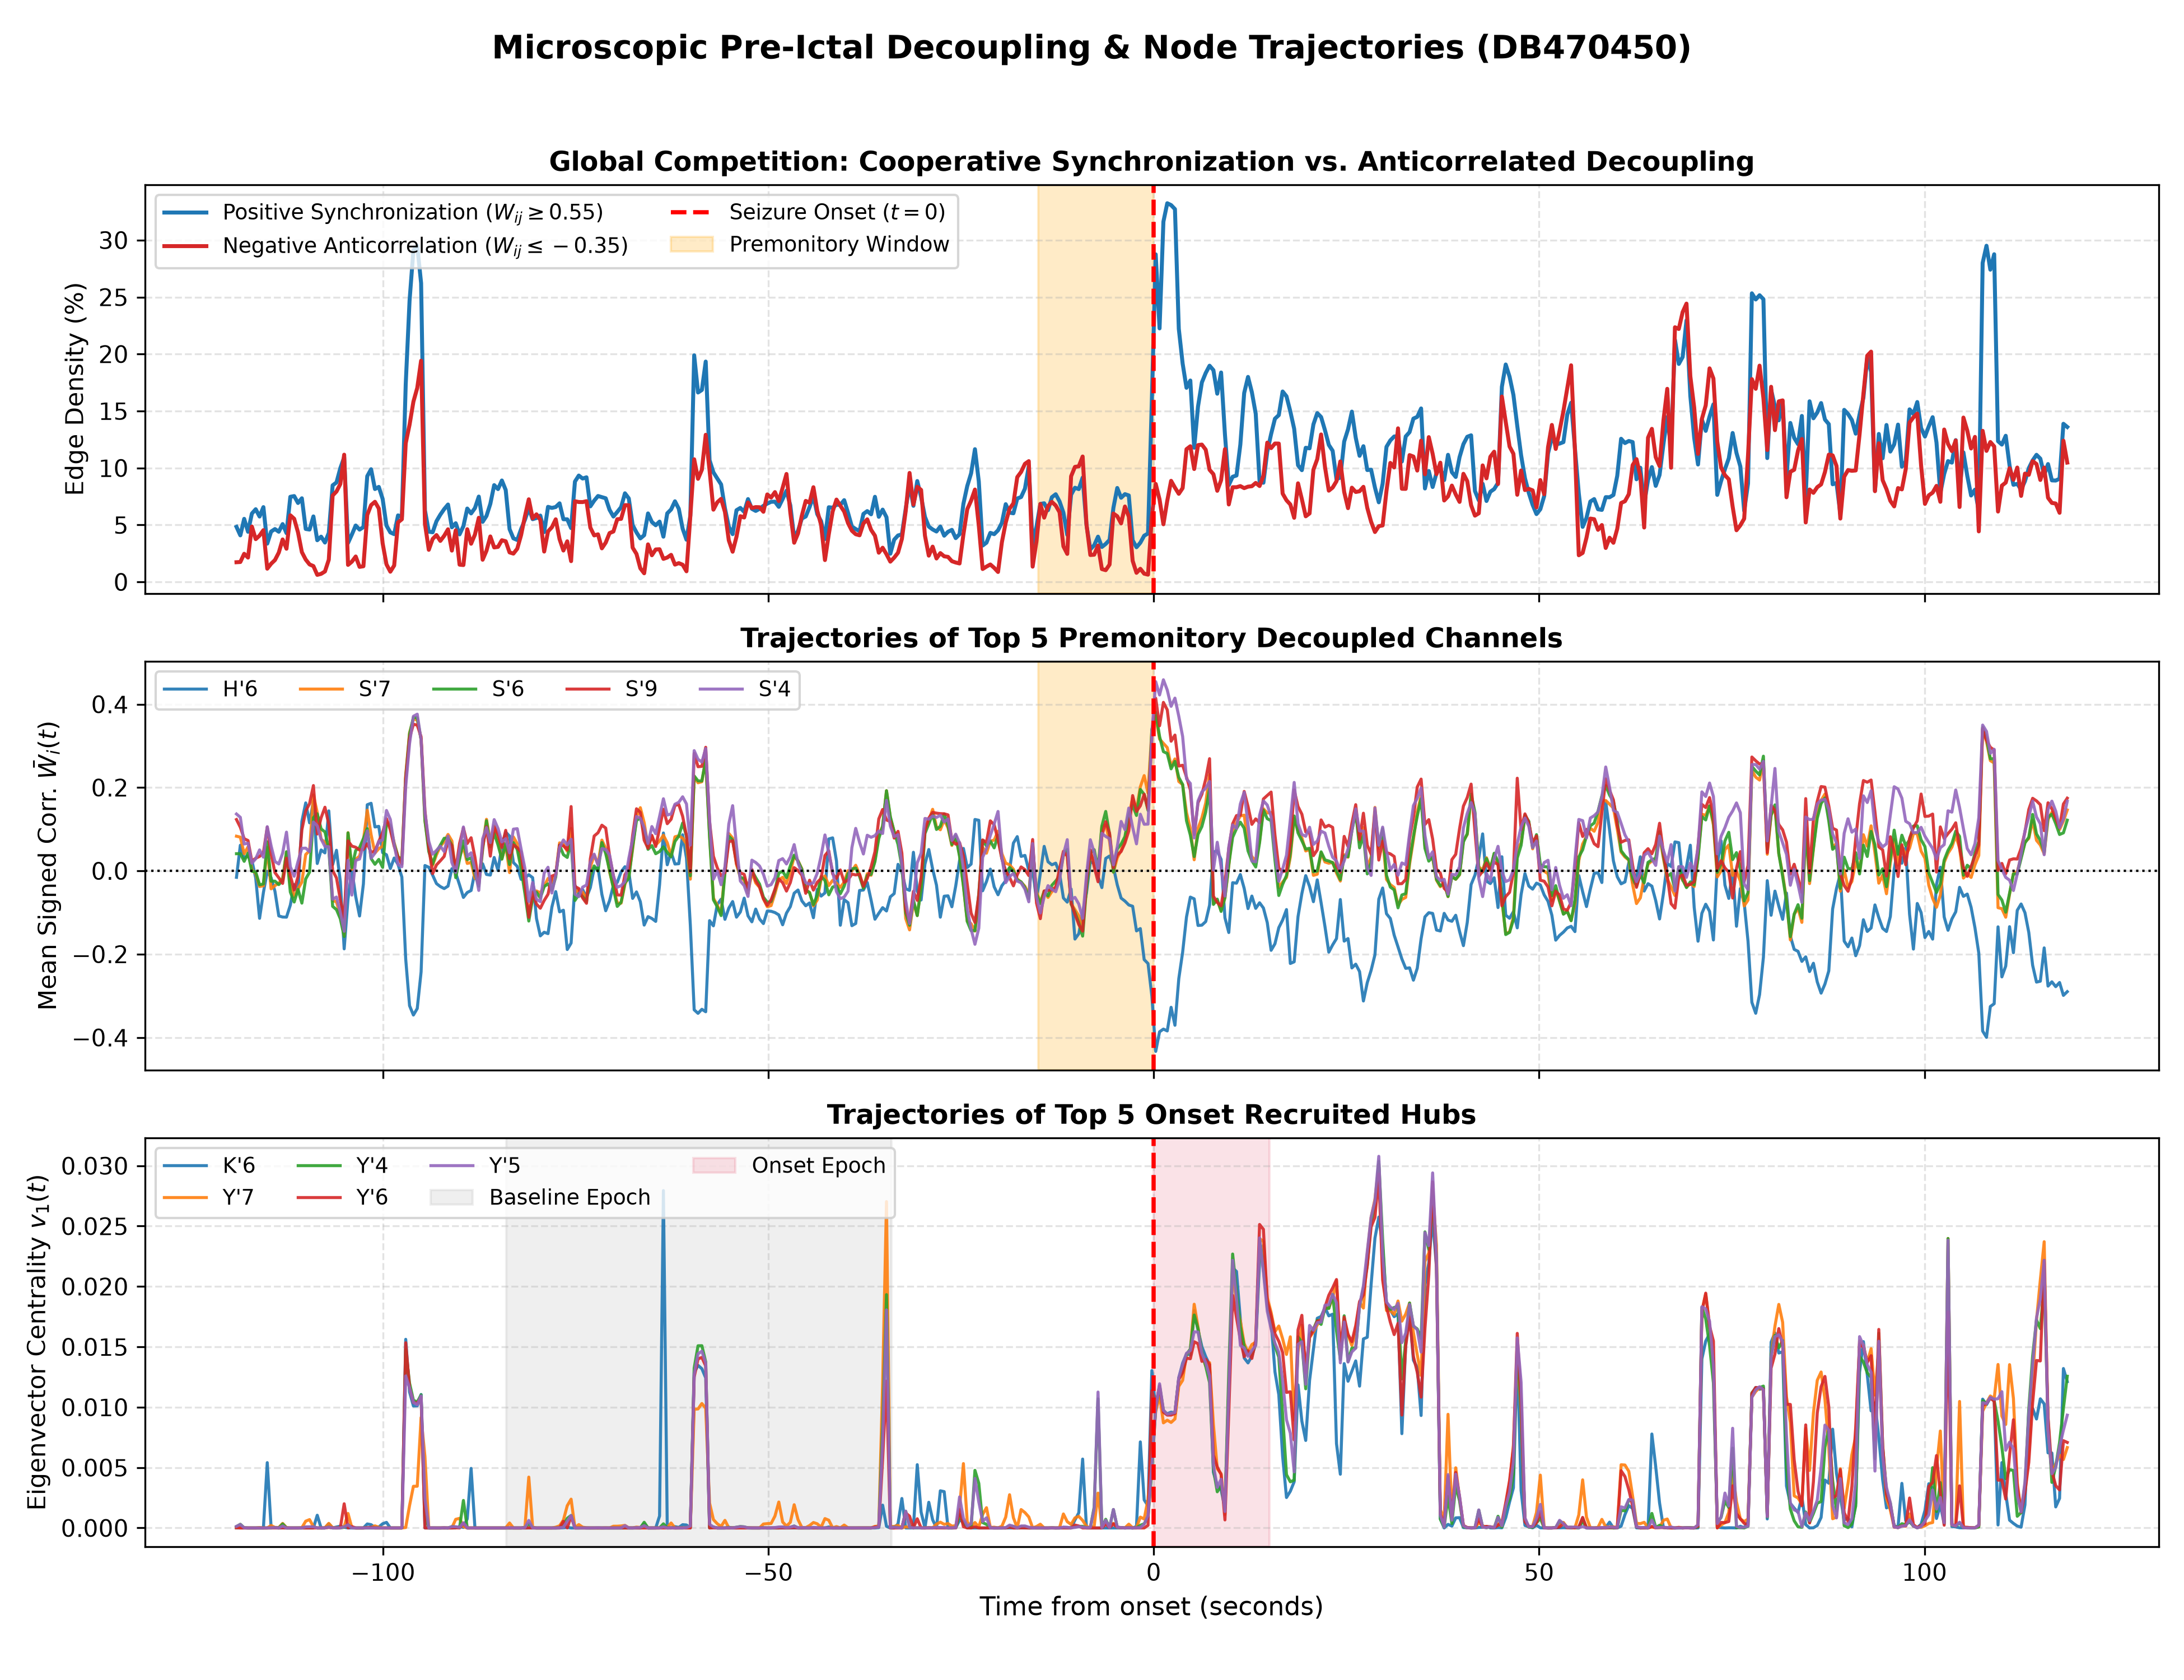
\includegraphics[width=0.9\textwidth]{img/DB470450/micro_premonitory_decoupling.png}
    \caption{Microscopic pre-ictal decoupling and nodal centrality trajectories in recording \texttt{DB470450} ($\theta = 0.55$). Top: Global edge density competition between cooperative synchronization ($W_{ij} \geq 0.55$, blue) and negative anticorrelation ($W_{ij} \leq -0.35$, red), highlighting the Premonitory Window ($[-15, 0]\text{ s}$, orange shading). Middle: Mean signed correlation trajectories $\bar{W}_i(\tau)$ of the top 5 premonitory decoupled channels (\texttt{H'6}, \texttt{S'7}, \texttt{S'6}, \texttt{S'9}, \texttt{S'4}). Bottom: Leading eigenvector centrality trajectories $v_{1,i}(\tau)$ of the top 5 onset-recruited hubs (\texttt{K'6}, \texttt{Y'7}, \texttt{Y'4}, \texttt{Y'6}, \texttt{Y'5}), contrasting the quiet Baseline Epoch ($[-84, -34]\text{ s}$, grey shading) against the Onset Epoch ($[0, +15]\text{ s}$, pink shading).}
    \label{fig:act3_trajectories}
\end{figure}

Inspecting the middle and bottom panels of Figure~\ref{fig:act3_trajectories} reveals a remarkable dynamical dichotomy across the critical transition:
\begin{itemize}
    \item \textbf{Premonitory Decoupling and Bifurcation at $t = 0\text{ s}$ (Middle Panel):} The five channels exhibiting the strongest pre-ictal detachment belong exclusively to two anatomical electrode shafts: contact \texttt{H'6} and a contiguous cluster on shaft \texttt{S'} (\texttt{S'7}, \texttt{S'6}, \texttt{S'9}, \texttt{S'4}). Inside the Premonitory Window ($\tau \in [-15, 0]\text{ s}$, orange shading), all five contacts dip into negative mean correlation ($\bar{W}_i(\tau) \approx -0.15\text{ to } -0.20$), confirming active functional isolation prior to seizure onset. Crucially, as the system crosses $t = 0\text{ s}$, their trajectories undergo a striking bifurcation: the \texttt{S'} contacts (\texttt{S'4}, \texttt{S'6}, \texttt{S'7}, \texttt{S'9}) rapidly invert their phase and shoot upward to $\bar{W}_i \approx +0.45$, joining the cooperative ictal syncytium; conversely, contact \texttt{H'6} (blue trace) plunges sharply downward to $\bar{W}_{\text{H'6}} \approx -0.43$ and remains locked in persistent counter-phase throughout the entire seizure.
    \item \textbf{Onset Centrality Surge and Baseline Robustness (Bottom Panel):} The bottom panel tracks $v_{1,i}(\tau)$ for the five strongest cooperative hubs (\texttt{K'6}, \texttt{Y'7}, \texttt{Y'4}, \texttt{Y'6}, \texttt{Y'5}). Notice how our automated baseline calibration placed the reference window ($\mathcal{E}_{\text{base}} = [-84, -34]\text{ s}$, grey shading) in a predominantly quiet region, avoiding the large inter-ictal burst at $\tau \approx -95\text{ s}$ and minimizing the impact of the brief spike at $\tau \approx -59\text{ s}$. Whereas $v_{1,i}(\tau)$ remains pinned near zero across the baseline, it jumps immediately at $t = 0\text{ s}$ (pink Onset Epoch) to a sustained high-centrality plateau ($v_{1,i} \in [0.010, 0.030]$ lasting until $\tau \approx +40\text{ s}$), identifying shafts \texttt{K'} and \texttt{Y'} as the core structural backbone of the ictal Giant Connected Component.
\end{itemize}

To synthesize these two orthogonal dynamical behaviors across the entire array of $N$ electrodes, Figure~\ref{fig:act3_rolemap} pairs the ranked bar chart of top onset hubs (left panel) with the two-dimensional \textbf{Microscopic Node Role Map} (right panel).

\begin{figure}[htbp]
    \centering
    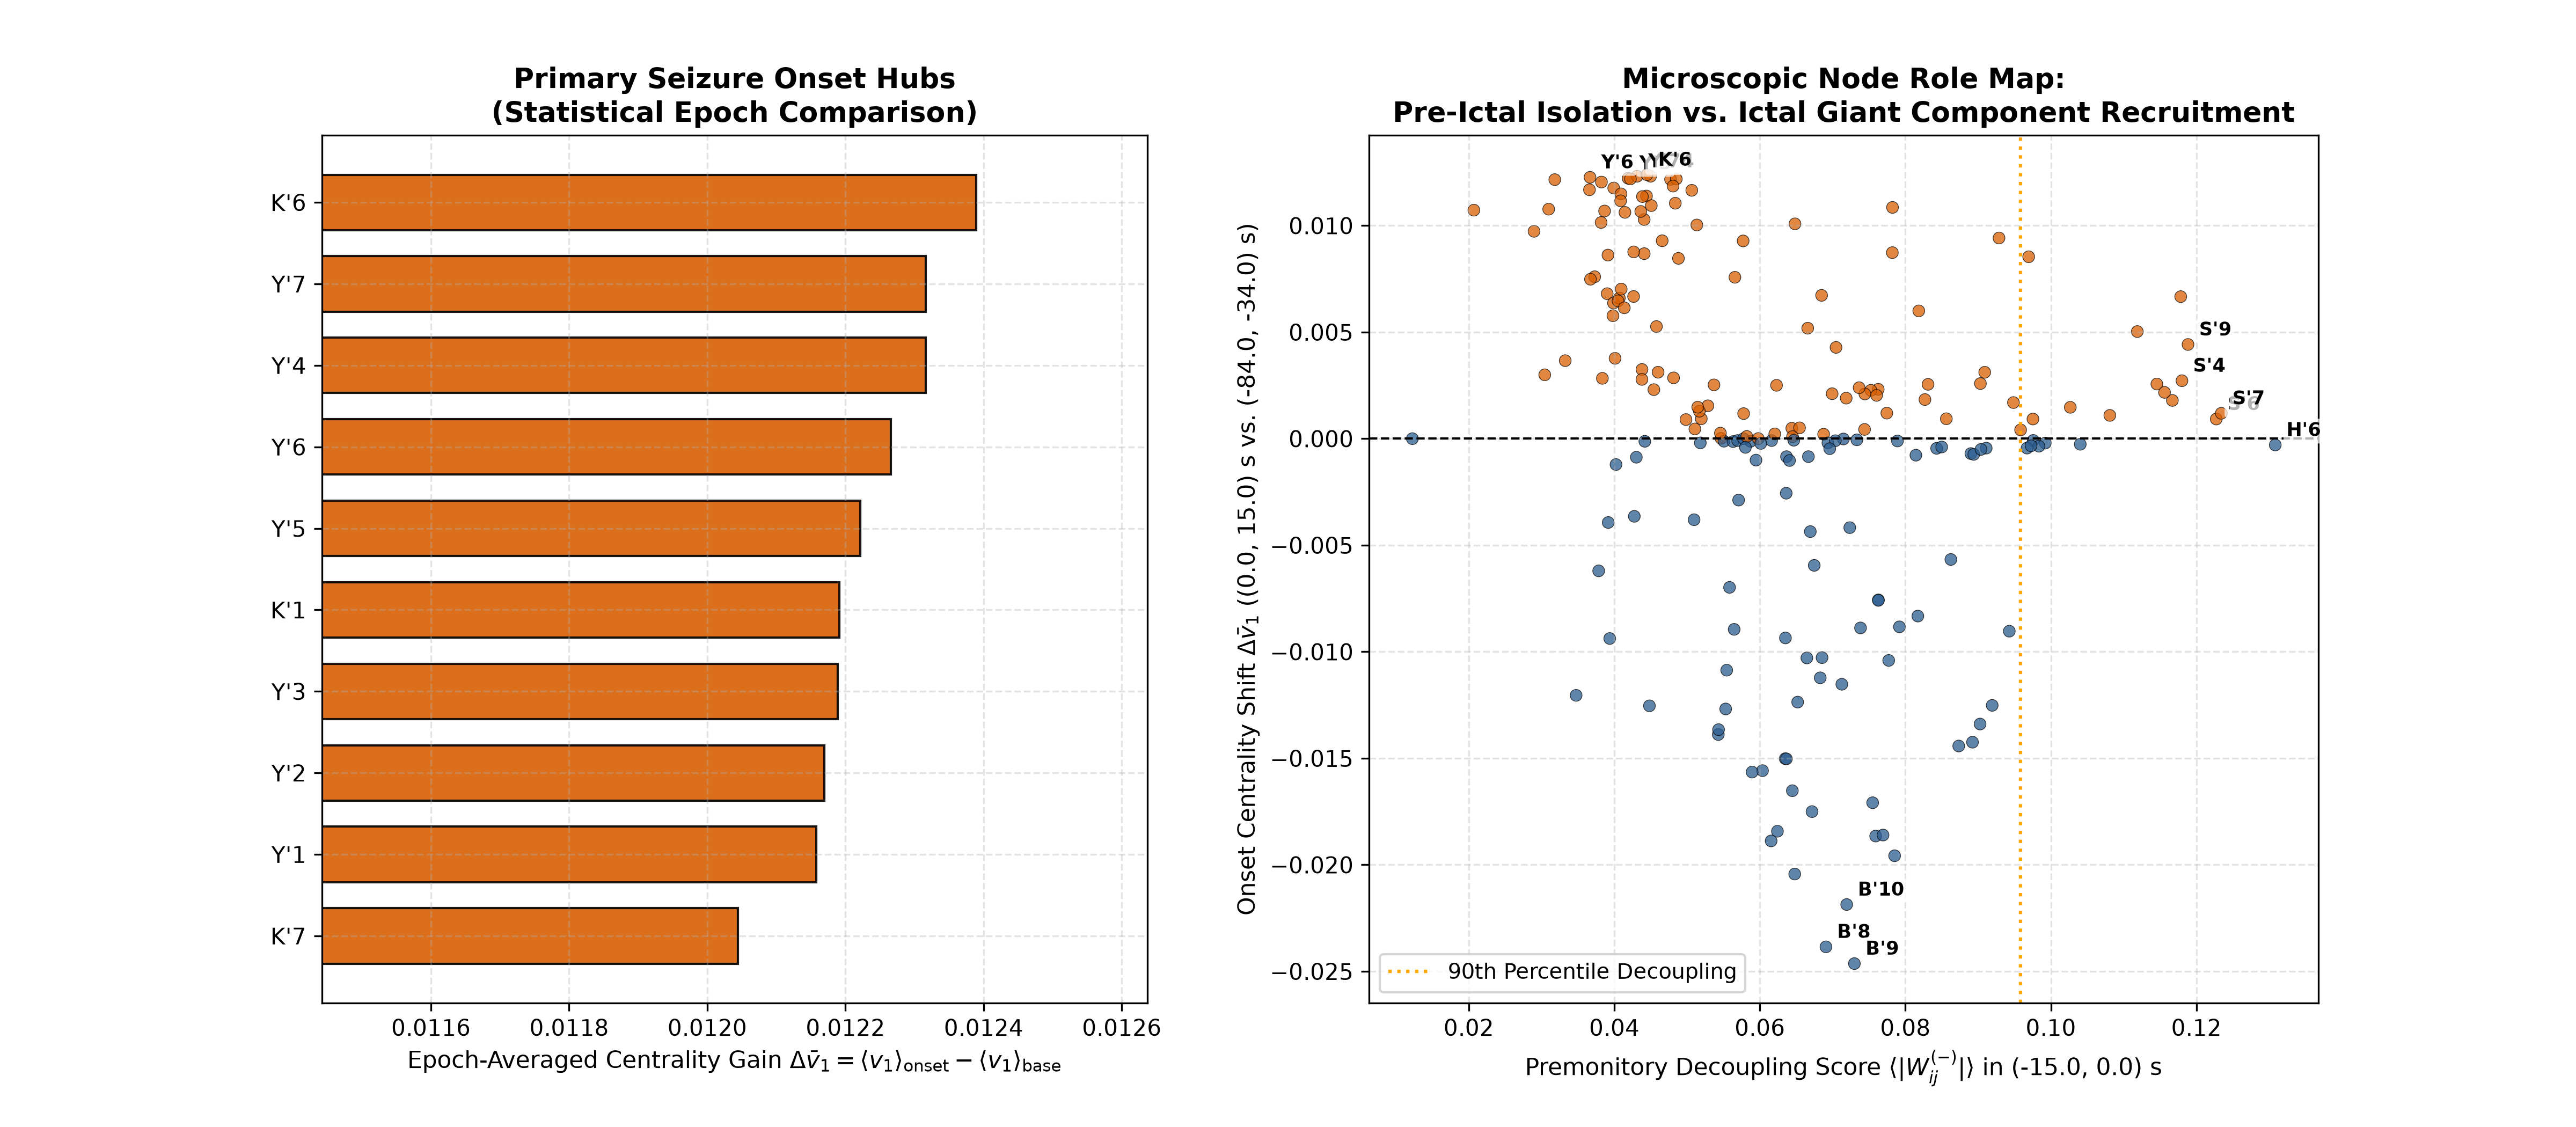
\includegraphics[width=0.9\textwidth]{img/DB470450/micro_hub_recruitment_and_roles.png}
    \caption{Epoch-averaged hub ranking and 2D Microscopic Node Role Map for recording \texttt{DB470450}. Left: Top 10 primary seizure onset hubs ranked by epoch-averaged eigenvector centrality gain $\Delta \bar{v}_{1,i} = \langle v_{1,i}\rangle_{\text{onset}} - \langle v_{1,i}\rangle_{\text{base}}$ (horizontal axis rescaled to $[0.0115, 0.0126]$ to resolve fine nodal hierarchy). Right: Joint scatter distribution of all intracranial channels plotting Premonitory Decoupling Score $\langle d_i^{(-)}\rangle_{\text{prem}}$ in $[-15, 0]\text{ s}$ (x-axis) against Onset Centrality Shift $\Delta \bar{v}_{1,i}$ (y-axis). The vertical orange dotted line marks the 90th percentile of premonitory decoupling; the horizontal black dashed line separates net onset hub recruitment ($\Delta \bar{v}_1 > 0$, orange circles) from centrality suppression ($\Delta \bar{v}_1 < 0$, blue circles).}
    \label{fig:act3_rolemap}
\end{figure}

The 2D Functional Role Map in Figure~\ref{fig:act3_rolemap} (right panel) spontaneously partitions the intracranial electrode contacts into four physically and clinically interpretable dynamical regimes:
\begin{enumerate}
    \item \textbf{Premonitory Seizure Initiators (Upper-Right Quadrant, high $\langle d_i^{(-)}\rangle_{\text{prem}} > 0.096$, $\Delta \bar{v}_1 > 0$):} Populated by the contiguous shaft \texttt{S'} cluster (\texttt{S'9}, \texttt{S'4}, \texttt{S'7}, \texttt{S'6}, with decoupling scores reaching $0.115\text{--}0.125$ and positive centrality gain $\Delta \bar{v}_1 \in [+0.001, +0.007]$). These nodes directly validate the clinical pre-ictal decoupling hypothesis: they actively detach from the physiological network in the $15\text{ seconds}$ prior to onset and subsequently transition into cooperative hubs that help drive the ictal cascade.
    \item \textbf{Primary Ictal Amplifiers / Core Hubs (Upper-Left Quadrant, low $\langle d_i^{(-)}\rangle_{\text{prem}} \approx 0.035\text{--}0.050$, maximum $\Delta \bar{v}_1 \approx +0.0120\text{--}0.0124$):} Dominated by a tightly clustered group of contacts along shafts \texttt{K'} and \texttt{Y'}—led by \texttt{K'6} ($\Delta \bar{v}_1 = 0.0124$), followed closely by \texttt{Y'7}, \texttt{Y'4}, \texttt{Y'6}, \texttt{Y'5}, \texttt{K'1}, \texttt{Y'3}, \texttt{Y'2}, \texttt{Y'1}, and \texttt{K'7} (resolved in the left bar chart). These channels do not exhibit premonitory counter-phase isolation prior to $t = 0\text{ s}$; rather, they act as massive cortical resonators that are explosively recruited at $t = 0\text{ s}$ to form the dominant synchronous core of the Giant Connected Component.
    \item \textbf{Persistent Counter-Phase Pole (Far-Right Boundary along $\Delta \bar{v}_1 \approx 0$):} Uniquely occupied by contact \texttt{H'6}, which achieves the highest premonitory decoupling score in the entire brain ($\langle d_{\text{H'6}}^{(-)}\rangle_{\text{prem}} \approx 0.133$) while maintaining $\Delta \bar{v}_1 \approx 0.000$. Because $\mathbf{v}_1(\tau)$ is computed strictly on cooperative positive links ($W_{ij} \geq 0.55$), \texttt{H'6} gains zero positive centrality at onset precisely because it remains locked in strong anti-phase oscillation ($\bar{W}_{\text{H'6}} < 0$) against the Giant Component throughout the seizure.
    \item \textbf{Demoted Background Nodes (Lower Half-Plane, $\Delta \bar{v}_1 < 0$, blue circles):} Contacts such as \texttt{B'9}, \texttt{B'8}, and \texttt{B'10} ($\Delta \bar{v}_1 \approx -0.021\text{ to }-0.024$), which participated in resting-state baseline connectivity during $\mathcal{E}_{\text{base}}$ but lose their relative share of network centrality at $t = 0\text{ s}$ as the $L_1$-normalized eigenvector weight concentrates onto the ictal hubs \texttt{K'} and \texttt{Y'}.
\end{enumerate}

\subsection{Critical Assessment and Methodological Caveats of Role Mapping}
Although the 2D Functional Role Map provides a clean, data-driven separation between premonitory decoupling channels (\texttt{S'}, \texttt{H'6}) and onset amplification hubs (\texttt{K'}, \texttt{Y'}), caution is warranted when interpreting these topological roles in a clinical or predictive context:
\begin{itemize}
    \item \textbf{Retrospective vs.\ Prospective Prediction:} The Premonitory Window $\mathcal{E}_{\text{prem}} = [-15, 0]\text{ s}$ is defined retrospectively relative to a known onset $t = 0\text{ s}$. Moreover, as visible in the middle panel of Figure~\ref{fig:act3_trajectories}, brief inter-ictal bursts (e.g., at $\tau \approx -95\text{ s}$ and $-59\text{ s}$) also trigger transient counter-phase deflections in \texttt{H'6} and positive spikes in \texttt{S'} without evolving into a seizure. Thus, pre-ictal decoupling alone is a necessary dynamical precursor of the transition, but cannot be claimed as a standalone, zero-false-positive prospective seizure predictor without testing over multi-hour inter-ictal recordings.
    \item \textbf{Zero-Lag Correlation Ambiguity:} Because Pearson correlation $W_{ij}(\tau)$ is a symmetric, zero-lag measure ($W_{ij} = W_{ji}$), observing $\bar{W}_{\text{H'6}} < 0$ cannot distinguish whether contact \texttt{H'6} is actively generating inhibitory counter-phase output or merely recording the inverted dipole pole of a nearby cortical generator.
\end{itemize}

\section{Cross-Patient Cohort Robustness and Parameter Calibration}
\label{sec:cohort_robustness}

A fundamental requirement for any physical model of biological dynamics is generalizability across subjects. While Sections~\ref{sec:act1_macro}--\ref{sec:act3_micro} detailed the multiscale cascade on our primary reference recording (\texttt{DB470450}), extending the pipeline across the full clinical dataset revealed that raw, uncalibrated topological metrics are highly sensitive to inter-patient experimental variability. Specifically, evaluating the cohort highlighted three sources of heterogeneity that must be controlled to uncover the universal signature of the phase transition:

\begin{enumerate}
    \item \textbf{Discrepancies Between Clinical and Electrophysiological Onset:} In our initial uncalibrated runs, while the \texttt{DB} recordings displayed sharp transitions near the nominal metadata timestamp, the remaining recordings exhibited seemingly noisy, uninterpretable pre-ictal profiles. In one recording, the macroscopic surge in synchronization occurred $30\text{--}40\text{ s}$ after the annotated marker; in another (e.g., \texttt{DQ0040WG}), strong synchronization bursts ($D^{+}(\tau) > 65\%$) invaded the nominal premonitory window $[-15, 0]\text{ s}$ well before the annotated $t = 0\text{ s}$. Applying the automated step-gradient detector introduced in Equation~(\ref{eq:onset_detector}) resolved this anomaly: clinical metadata often log the delayed behavioral manifestation of the seizure (\textit{clinical onset}) rather than the deep intracranial bifurcation (\textit{electrophysiological onset}). Re-centering $t = 0\text{ s}$ on the objective energy-synchronization jump restored the sharp step transition across all recordings.

    \item \textbf{Implantation Density and Sub-Critical Threshold Scaling:} Because each patient receives a personalized stereotactic implantation tailored to their suspected clinical semiology, the spatial density of electrode contacts varies across recordings. In densely sampled implants (such as \texttt{DQ0040WG}), applying the default threshold $\theta = 0.50$ resulted in an overly dense baseline graph ($D^{+}_{\text{base}} \approx 15\text{--}25\%$), causing frequent spurious spikes in leading eigenvector centrality $v_{1,i}(\tau)$ prior to onset. Scaling the positive threshold $\theta \in [0.50, 0.65]$ via our data-driven criterion—enforcing a sub-critical baseline link density of $D^{+}_{\text{base}}(\theta) \approx 7\%$—successfully suppressed pre-ictal percolation noise and flattened the baseline centrality traces across the cohort.

    \item \textbf{Contamination from Extracranial Polygraphic Channels and Pre-Ictal Bursts:} Cross-patient inspection also exposed the critical impact of auxiliary channels and inter-ictal spikes. Prior to implementing the automated label filter (Section~\ref{sec:dataset_extraction}), polygraphic reference channels (such as \texttt{POL-7} in recording \texttt{DQ0040WG}) consistently ranked among the top 5 premonitory decoupled nodes, driven by subtle pre-ictal muscle or autonomic artifacts that correlated negatively with cortical potentials. Removing \texttt{POL}/\texttt{ECG} channels and automatically shifting the $50\text{ s}$ Baseline Epoch $\mathcal{E}_{\text{base}}$ to avoid isolated inter-ictal bursts ensured that both the bar rankings and the 2D Role Maps strictly reflected genuine intracranial neural populations (such as hippocampal \texttt{H} and cortical \texttt{G}/\texttt{D}/\texttt{E} shafts).
\end{enumerate}

Once these three objective calibration steps are applied, the qualitative phenomenology of the transition proves remarkably invariant across recordings: every seizure in the cohort is characterized by a sub-critical modular baseline ($Q \approx 0.6\text{--}0.8$), a premonitory counter-phase detachment of specific focal contacts in the $[-15, 0]\text{ s}$ window, and an abrupt percolation collapse at $t = 0\text{ s}$ where $S(\tau) \to 1$ and $\chi(\tau)$ peaks.

The complete multiscale graphical outputs (Macroscopic Percolation, Mesoscopic Modularity Collapse, and Microscopic Node Role Maps) for the remaining cohort recordings are reported in Appendix~\ref{app:cohort_figures}. Across all subjects, the calibrated topological pipeline consistently recovers the transition from pre-ictal modular segregation and focal counter-phase decoupling to global ictal percolation.